\documentclass[12pt]{article}    
\usepackage{ucs} 
\usepackage[utf8x]{inputenc}
\usepackage[russian]{babel}  
\usepackage{float}
\title{Псевдоэксперимент №1}
\author{Хафизов Фанис}
\usepackage[pdftex]{graphicx}
\usepackage{multirow}

\begin{document}
	\begin{figure}
		\centering
		
\includegraphics[width=0.3\linewidth]{logo}
	\end{figure}
	\maketitle
	\newpage
	\section{Теория}
	\begin{figure}[H]
		\centering
		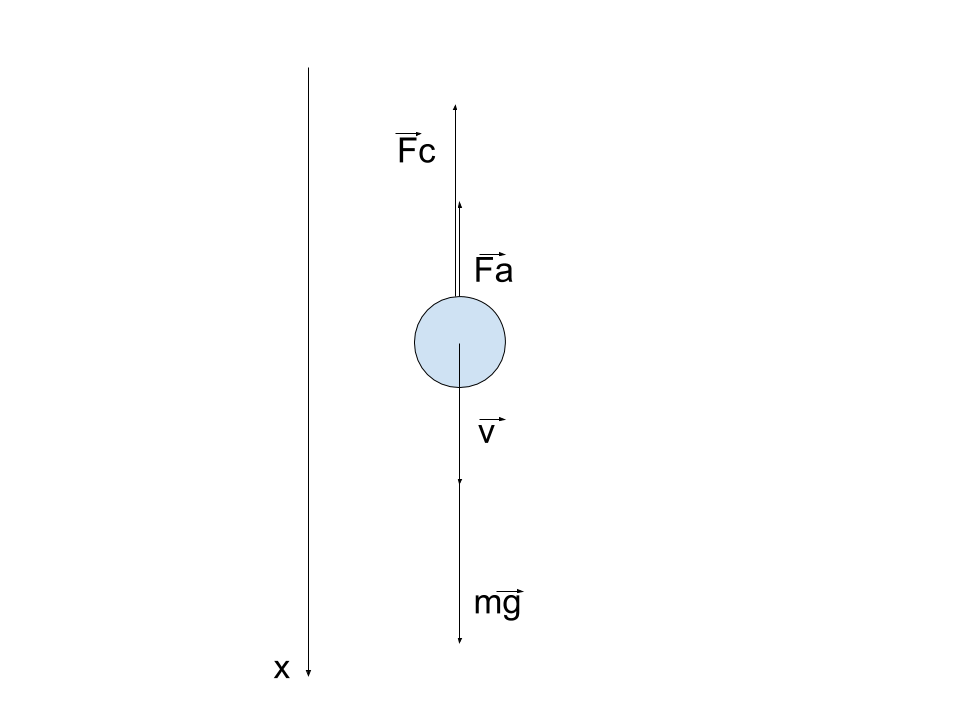
\includegraphics[width=1.0\linewidth]{pic}
	\end{figure}
	Запишем уравнение второго закона Ньютона:
	$$\vec{F_c}+\vec{F_a}+m\vec{g}=0$$
	$$Ox:mg-F_a-F_c=0$$
	$$F_c=A\eta vd$$
	$$F_a=\rho_wgV=\rho_wg\frac{4}{3}\pi\frac{d^3}{8}=\rho_wg\frac{\pi d^3}{6}$$
	$$m=\rho_c V=\rho\frac{4\pi d^3}{3\cdot8}=\rho_c\frac{\pi d^3}{6}$$
	$$(\rho_c-\rho_w)g\frac{d^3}{6}=A\eta\frac{l}{\tau}d$$
	$$\tau=\frac{6A\eta l}{gd^2(\rho_c-\rho_w)}$$
	\section{Расчеты}
	Построим график зависимости $\tau$ от $\frac{1}{d^2}$.
	
\begin{table}[H]
\begin{tabular}{|r|r|r|r|r|r|r|r|}
\hline
\multicolumn{1}{|l|}{\multirow{2}{*}{d, мм}} & \multicolumn{5}{l|}{Время движения, с}                                                                                                                   & \multicolumn{1}{l|}{}                   & \multicolumn{1}{l|}{}                                   \\ \cline{2-6}
\multicolumn{1}{|l|}{}                       & \multicolumn{1}{l|}{$\tau_1$} & \multicolumn{1}{l|}{$\tau_2$} & \multicolumn{1}{l|}{$\tau_3$} & \multicolumn{1}{l|}{$\tau_4$} & \multicolumn{1}{l|}{$\tau_5$} & \multicolumn{1}{l|}{$\overline{\tau}$} & \multicolumn{1}{l|}{$1/d^2$, м$^{-2}$} \\ \hline
1,00                                         & 60,94                        & 60,73                        & 60,54                        & 60,81                        & 60,55                        & 60,714                                  & 1 000 000,00                                            \\ \hline
4,39                                         & 5,58                         & 5,73                         & 5,45                         & 5,32                         & 5,44                         & 5,504                                   & 51 888,48                                               \\ \hline
2,02                                         & 15,94                        & 15,73                        & 15,55                        & 15,92                        & 15,43                        & 15,714                                  & 245 074,01                                              \\ \hline
2,70                                         & 8,93                         & 8,63                         & 9,14                         & 8,99                         & 9,18                         & 8,974                                   & 137 174,21                                              \\ \hline
3,70                                         & 4,94                         & 4,73                         & 4,92                         & 4,39                         & 4,34                         & 4,664                                   & 73 046,02                                               \\ \hline
3,21                                         & 6,37                         & 6,26                         & 6,41                         & 6,23                         & 6,13                         & 6,280                                   & 97 048,75                                               \\ \hline
3,35                                         & 5,27                         & 5,25                         & 5,62                         & 5,76                         & 5,71                         & 5,522                                   & 89 106,71                                               \\ \hline
\end{tabular}
\end{table}
	\begin{figure}[H]
		\centering
		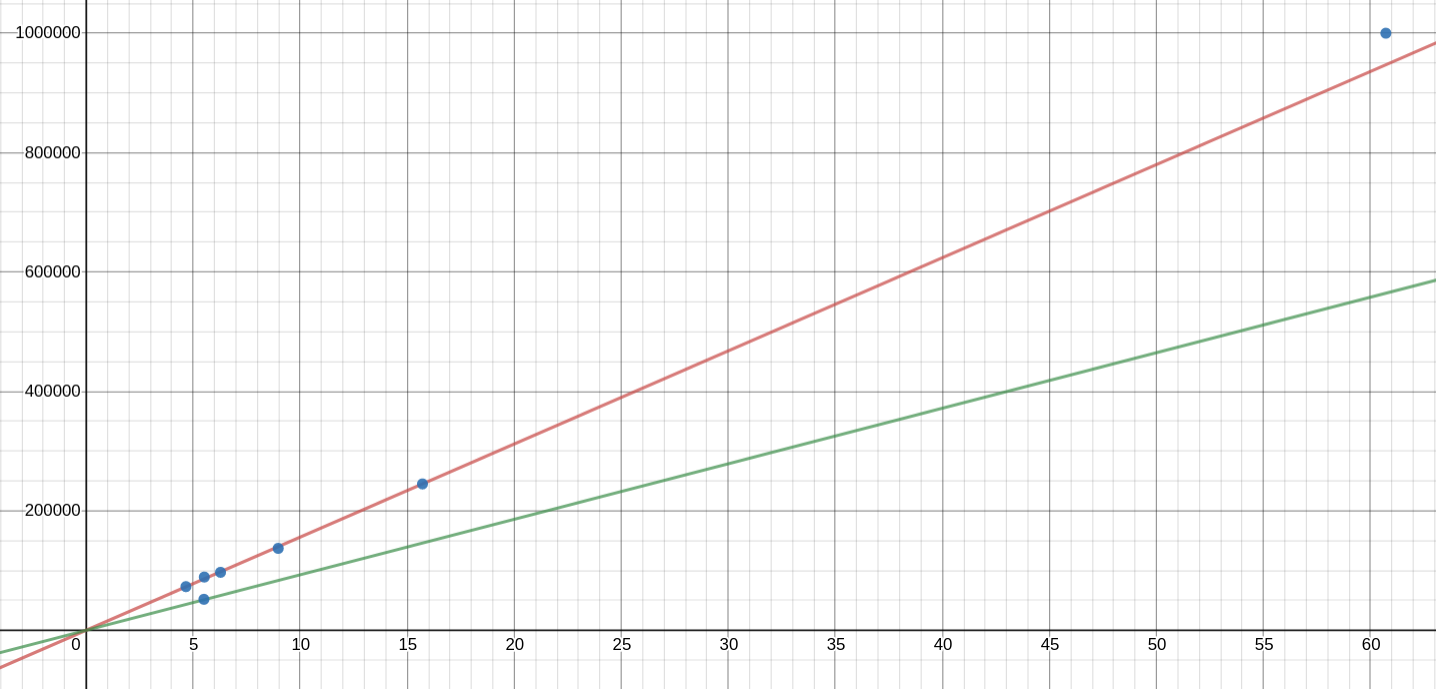
\includegraphics[width=\linewidth]{graph}
	\end{figure}
	Как мы видим, все точки, кроме (5,504; 51888,48), лежат на одной прямой. Значит, шарик под номером 2 отличается от всех остальных и у него другая плотность. Угловые коэффициенты графиков равны 15600 для свинцового и 9300 для отличающегося шарика соответственно.
	$$\frac{A\eta l}{g(\rho_c-\rho_w)}=15600$$
	$$\frac{A\eta l}{g(\rho_x-\rho_w)}=9300$$
	$$\frac{\rho_x-\rho_w}{\rho_c-\rho_w}=\frac{15600}{9300}$$	
	$\displaystyle\rho_x=\frac{15600}{9300}(\rho_c-\rho_w)+\rho_w=\frac{15600}{9300}(11,3-1,0)+1,0=18,27$\cyrg/\cyrs\cyrm$^3$
	\section{Расчет погрешностей}
	$$\varepsilon_{\rho_x}=\varepsilon_{\tau}+2\varepsilon_{d}=\sum\limits^7_{i=1}\sqrt{\frac{\sum\limits^5_{j=1}(\tau_{ij}-\overline{\tau_i})^2}{5\overline{\tau^2}}}+\sum\limits^7_{i=1}\frac{\Delta d}{d_i}=23,2\%$$
	$\Delta \rho_x=\rho_x\cdot \varepsilon_{\rho_x}=18,27\cdot0,232=4,24$г/см$^3$
	\section{Ответ}
	$\rho_x=(18,27\pm4,24)$г/см$^3$
\end{document}